\section{Event Unit}

\pulpino features a lightweight event and interrupt unit which supports
vectorized interrupts of up to 32 lines and event triggering of up to 32 input
lines. The interrupt and event lines are separately masked and buffered, see
Figure~\ref{fig:event_unit}.


\begin{figure}[H]
  \centering
  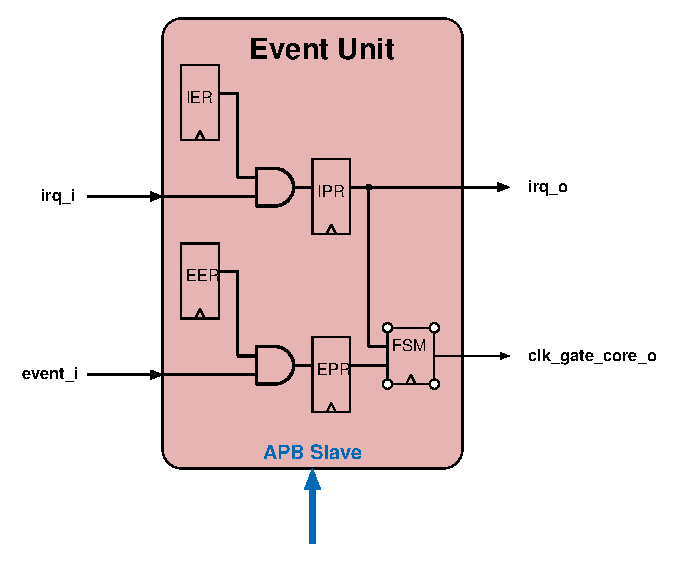
\includegraphics[width=0.6\textwidth]{./figures/event_unit}
  \caption{Event Unit.}
  \label{fig:event_unit}
\end{figure}

The current assignment of event and interrupt lines is given in
Figure~\ref{fig:event_lines}. Note that \signal{irq\_i} and \signal{event\_i}
are bound together.

\begin{figure}[H]
  \centering
  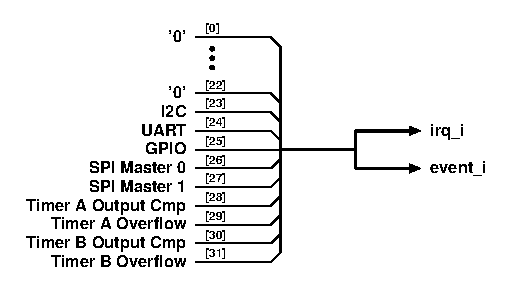
\includegraphics[width=0.6\textwidth]{./figures/event_lines}
  \caption{Event Lines.}
  \label{fig:event_lines}
\end{figure}


\regDesc{0x1A10\_4000}{0x0000\_0000}{IER (Interrupt Enable)}{
  \begin{bytefield}[rightcurly=.,endianness=big]{32}
  \bitheader{31,30,29,28,27,26,25,24,23,22,21,20,19,18,17,16,15,14,13,12,11,10,9,8,7,6,5,4,3,2,1,0} \\
  \begin{rightwordgroup}{IER}
    \bitbox{1}{\tiny E}
    \bitbox{1}{\tiny E}
    \bitbox{1}{\tiny E}
    \bitbox{1}{\tiny E}
    \bitbox{1}{\tiny E}
    \bitbox{1}{\tiny E}
    \bitbox{1}{\tiny E}
    \bitbox{1}{\tiny E}
    \bitbox{1}{\tiny E}
    \bitbox{1}{\tiny E}
    \bitbox{1}{\tiny E}
    \bitbox{1}{\tiny E}
    \bitbox{1}{\tiny E}
    \bitbox{1}{\tiny E}
    \bitbox{1}{\tiny E}
    \bitbox{1}{\tiny E}
    \bitbox{1}{\tiny E}
    \bitbox{1}{\tiny E}
    \bitbox{1}{\tiny E}
    \bitbox{1}{\tiny E}
    \bitbox{1}{\tiny E}
    \bitbox{1}{\tiny E}
    \bitbox{1}{\tiny E}
    \bitbox{1}{\tiny E}
    \bitbox{1}{\tiny E}
    \bitbox{1}{\tiny E}
    \bitbox{1}{\tiny E}
    \bitbox{1}{\tiny E}
    \bitbox{1}{\tiny E}
    \bitbox{1}{\tiny E}
    \bitbox{1}{\tiny E}
    \bitbox{1}{\tiny E}
  \end{rightwordgroup}\\
  \end{bytefield}
}{
  \regItem{Bit 31:0}{IER}{Interrupt Enable.\\
    Enable interrupts per line.
  }
}

\regDesc{0x1A10\_4004}{0x0000\_0000}{IPR (Interrupt Pending)}{
  \begin{bytefield}[rightcurly=.,endianness=big]{32}
  \bitheader{31,30,29,28,27,26,25,24,23,22,21,20,19,18,17,16,15,14,13,12,11,10,9,8,7,6,5,4,3,2,1,0} \\
  \begin{rightwordgroup}{IPR}
    \bitbox{1}{\tiny P}
    \bitbox{1}{\tiny P}
    \bitbox{1}{\tiny P}
    \bitbox{1}{\tiny P}
    \bitbox{1}{\tiny P}
    \bitbox{1}{\tiny P}
    \bitbox{1}{\tiny P}
    \bitbox{1}{\tiny P}
    \bitbox{1}{\tiny P}
    \bitbox{1}{\tiny P}
    \bitbox{1}{\tiny P}
    \bitbox{1}{\tiny P}
    \bitbox{1}{\tiny P}
    \bitbox{1}{\tiny P}
    \bitbox{1}{\tiny P}
    \bitbox{1}{\tiny P}
    \bitbox{1}{\tiny P}
    \bitbox{1}{\tiny P}
    \bitbox{1}{\tiny P}
    \bitbox{1}{\tiny P}
    \bitbox{1}{\tiny P}
    \bitbox{1}{\tiny P}
    \bitbox{1}{\tiny P}
    \bitbox{1}{\tiny P}
    \bitbox{1}{\tiny P}
    \bitbox{1}{\tiny P}
    \bitbox{1}{\tiny P}
    \bitbox{1}{\tiny P}
    \bitbox{1}{\tiny P}
    \bitbox{1}{\tiny P}
    \bitbox{1}{\tiny P}
    \bitbox{1}{\tiny P}
  \end{rightwordgroup}\\
  \end{bytefield}
}{
  \regItem{Bit 31:0}{IPR}{Interrupt Pending.\\
    Write/read pending interrupts per line.
  }
}

\regDesc{0x1A10\_4008}{0x0000\_0000}{ISP (Interrupt Set Pending)}{
  \begin{bytefield}[rightcurly=.,endianness=big]{32}
  \bitheader{31,30,29,28,27,26,25,24,23,22,21,20,19,18,17,16,15,14,13,12,11,10,9,8,7,6,5,4,3,2,1,0} \\
  \begin{rightwordgroup}{ISP}
    \bitbox{1}{\tiny S}
    \bitbox{1}{\tiny S}
    \bitbox{1}{\tiny S}
    \bitbox{1}{\tiny S}
    \bitbox{1}{\tiny S}
    \bitbox{1}{\tiny S}
    \bitbox{1}{\tiny S}
    \bitbox{1}{\tiny S}
    \bitbox{1}{\tiny S}
    \bitbox{1}{\tiny S}
    \bitbox{1}{\tiny S}
    \bitbox{1}{\tiny S}
    \bitbox{1}{\tiny S}
    \bitbox{1}{\tiny S}
    \bitbox{1}{\tiny S}
    \bitbox{1}{\tiny S}
    \bitbox{1}{\tiny S}
    \bitbox{1}{\tiny S}
    \bitbox{1}{\tiny S}
    \bitbox{1}{\tiny S}
    \bitbox{1}{\tiny S}
    \bitbox{1}{\tiny S}
    \bitbox{1}{\tiny S}
    \bitbox{1}{\tiny S}
    \bitbox{1}{\tiny S}
    \bitbox{1}{\tiny S}
    \bitbox{1}{\tiny S}
    \bitbox{1}{\tiny S}
    \bitbox{1}{\tiny S}
    \bitbox{1}{\tiny S}
    \bitbox{1}{\tiny S}
    \bitbox{1}{\tiny S}
  \end{rightwordgroup}\\
  \end{bytefield}
}{
  \regItem{Bit 31:0}{ISP}{Interrupt Set Pending.\\
    Set interrupt pending register per line. By setting a bit here, an interrupt
    will be triggered on the selected line(s).
  }
}

\regDesc{0x1A10\_400C}{0x0000\_0000}{ICP (Interrupt Clear Pending)}{
  \begin{bytefield}[rightcurly=.,endianness=big]{32}
  \bitheader{31,30,29,28,27,26,25,24,23,22,21,20,19,18,17,16,15,14,13,12,11,10,9,8,7,6,5,4,3,2,1,0} \\
  \begin{rightwordgroup}{ICP}
    \bitbox{1}{\tiny C}
    \bitbox{1}{\tiny C}
    \bitbox{1}{\tiny C}
    \bitbox{1}{\tiny C}
    \bitbox{1}{\tiny C}
    \bitbox{1}{\tiny C}
    \bitbox{1}{\tiny C}
    \bitbox{1}{\tiny C}
    \bitbox{1}{\tiny C}
    \bitbox{1}{\tiny C}
    \bitbox{1}{\tiny C}
    \bitbox{1}{\tiny C}
    \bitbox{1}{\tiny C}
    \bitbox{1}{\tiny C}
    \bitbox{1}{\tiny C}
    \bitbox{1}{\tiny C}
    \bitbox{1}{\tiny C}
    \bitbox{1}{\tiny C}
    \bitbox{1}{\tiny C}
    \bitbox{1}{\tiny C}
    \bitbox{1}{\tiny C}
    \bitbox{1}{\tiny C}
    \bitbox{1}{\tiny C}
    \bitbox{1}{\tiny C}
    \bitbox{1}{\tiny C}
    \bitbox{1}{\tiny C}
    \bitbox{1}{\tiny C}
    \bitbox{1}{\tiny C}
    \bitbox{1}{\tiny C}
    \bitbox{1}{\tiny C}
    \bitbox{1}{\tiny C}
    \bitbox{1}{\tiny C}
  \end{rightwordgroup}\\
  \end{bytefield}
}{
  \regItem{Bit 31:0}{ICP}{Interrupt Clear Pending.\\
    Clear pending interrupt. By setting a bit here, a pending interrupt will be
    cleared.
  }
}

\regDesc{0x1A10\_4010}{0x0000\_0000}{EER (Event Enable)}{
  \begin{bytefield}[rightcurly=.,endianness=big]{32}
  \bitheader{31,30,29,28,27,26,25,24,23,22,21,20,19,18,17,16,15,14,13,12,11,10,9,8,7,6,5,4,3,2,1,0} \\
  \begin{rightwordgroup}{EER}
    \bitbox{1}{\tiny E}
    \bitbox{1}{\tiny E}
    \bitbox{1}{\tiny E}
    \bitbox{1}{\tiny E}
    \bitbox{1}{\tiny E}
    \bitbox{1}{\tiny E}
    \bitbox{1}{\tiny E}
    \bitbox{1}{\tiny E}
    \bitbox{1}{\tiny E}
    \bitbox{1}{\tiny E}
    \bitbox{1}{\tiny E}
    \bitbox{1}{\tiny E}
    \bitbox{1}{\tiny E}
    \bitbox{1}{\tiny E}
    \bitbox{1}{\tiny E}
    \bitbox{1}{\tiny E}
    \bitbox{1}{\tiny E}
    \bitbox{1}{\tiny E}
    \bitbox{1}{\tiny E}
    \bitbox{1}{\tiny E}
    \bitbox{1}{\tiny E}
    \bitbox{1}{\tiny E}
    \bitbox{1}{\tiny E}
    \bitbox{1}{\tiny E}
    \bitbox{1}{\tiny E}
    \bitbox{1}{\tiny E}
    \bitbox{1}{\tiny E}
    \bitbox{1}{\tiny E}
    \bitbox{1}{\tiny E}
    \bitbox{1}{\tiny E}
    \bitbox{1}{\tiny E}
    \bitbox{1}{\tiny E}
  \end{rightwordgroup}\\
  \end{bytefield}
}{
  \regItem{Bit 31:0}{EER}{Event Enable.\\
    Enable events per line.
  }
}

\regDesc{0x1A10\_4014}{0x0000\_0000}{EPR (Event Pending)}{
  \begin{bytefield}[rightcurly=.,endianness=big]{32}
  \bitheader{31,30,29,28,27,26,25,24,23,22,21,20,19,18,17,16,15,14,13,12,11,10,9,8,7,6,5,4,3,2,1,0} \\
  \begin{rightwordgroup}{EPR}
    \bitbox{1}{\tiny P}
    \bitbox{1}{\tiny P}
    \bitbox{1}{\tiny P}
    \bitbox{1}{\tiny P}
    \bitbox{1}{\tiny P}
    \bitbox{1}{\tiny P}
    \bitbox{1}{\tiny P}
    \bitbox{1}{\tiny P}
    \bitbox{1}{\tiny P}
    \bitbox{1}{\tiny P}
    \bitbox{1}{\tiny P}
    \bitbox{1}{\tiny P}
    \bitbox{1}{\tiny P}
    \bitbox{1}{\tiny P}
    \bitbox{1}{\tiny P}
    \bitbox{1}{\tiny P}
    \bitbox{1}{\tiny P}
    \bitbox{1}{\tiny P}
    \bitbox{1}{\tiny P}
    \bitbox{1}{\tiny P}
    \bitbox{1}{\tiny P}
    \bitbox{1}{\tiny P}
    \bitbox{1}{\tiny P}
    \bitbox{1}{\tiny P}
    \bitbox{1}{\tiny P}
    \bitbox{1}{\tiny P}
    \bitbox{1}{\tiny P}
    \bitbox{1}{\tiny P}
    \bitbox{1}{\tiny P}
    \bitbox{1}{\tiny P}
    \bitbox{1}{\tiny P}
    \bitbox{1}{\tiny P}
  \end{rightwordgroup}\\
  \end{bytefield}
}{
  \regItem{Bit 31:0}{EPR}{Event Pending.\\
    Write/read pending events per line.
  }
}

\regDesc{0x1A10\_4018}{0x0000\_0000}{ESP (Event Set Pending)}{
  \begin{bytefield}[rightcurly=.,endianness=big]{32}
  \bitheader{31,30,29,28,27,26,25,24,23,22,21,20,19,18,17,16,15,14,13,12,11,10,9,8,7,6,5,4,3,2,1,0} \\
  \begin{rightwordgroup}{ESP}
    \bitbox{1}{\tiny S}
    \bitbox{1}{\tiny S}
    \bitbox{1}{\tiny S}
    \bitbox{1}{\tiny S}
    \bitbox{1}{\tiny S}
    \bitbox{1}{\tiny S}
    \bitbox{1}{\tiny S}
    \bitbox{1}{\tiny S}
    \bitbox{1}{\tiny S}
    \bitbox{1}{\tiny S}
    \bitbox{1}{\tiny S}
    \bitbox{1}{\tiny S}
    \bitbox{1}{\tiny S}
    \bitbox{1}{\tiny S}
    \bitbox{1}{\tiny S}
    \bitbox{1}{\tiny S}
    \bitbox{1}{\tiny S}
    \bitbox{1}{\tiny S}
    \bitbox{1}{\tiny S}
    \bitbox{1}{\tiny S}
    \bitbox{1}{\tiny S}
    \bitbox{1}{\tiny S}
    \bitbox{1}{\tiny S}
    \bitbox{1}{\tiny S}
    \bitbox{1}{\tiny S}
    \bitbox{1}{\tiny S}
    \bitbox{1}{\tiny S}
    \bitbox{1}{\tiny S}
    \bitbox{1}{\tiny S}
    \bitbox{1}{\tiny S}
    \bitbox{1}{\tiny S}
    \bitbox{1}{\tiny S}
  \end{rightwordgroup}\\
  \end{bytefield}
}{
  \regItem{Bit 31:0}{ESP}{Event Set Pending.\\
    Set event pending register per line. By setting a bit here, an event
    will be set on the selected line(s).
  }
}

\regDesc{0x1A10\_401C}{0x0000\_0000}{ECP (Event Clear Pending)}{
  \begin{bytefield}[rightcurly=.,endianness=big]{32}
  \bitheader{31,30,29,28,27,26,25,24,23,22,21,20,19,18,17,16,15,14,13,12,11,10,9,8,7,6,5,4,3,2,1,0} \\
  \begin{rightwordgroup}{ECP}
    \bitbox{1}{\tiny C}
    \bitbox{1}{\tiny C}
    \bitbox{1}{\tiny C}
    \bitbox{1}{\tiny C}
    \bitbox{1}{\tiny C}
    \bitbox{1}{\tiny C}
    \bitbox{1}{\tiny C}
    \bitbox{1}{\tiny C}
    \bitbox{1}{\tiny C}
    \bitbox{1}{\tiny C}
    \bitbox{1}{\tiny C}
    \bitbox{1}{\tiny C}
    \bitbox{1}{\tiny C}
    \bitbox{1}{\tiny C}
    \bitbox{1}{\tiny C}
    \bitbox{1}{\tiny C}
    \bitbox{1}{\tiny C}
    \bitbox{1}{\tiny C}
    \bitbox{1}{\tiny C}
    \bitbox{1}{\tiny C}
    \bitbox{1}{\tiny C}
    \bitbox{1}{\tiny C}
    \bitbox{1}{\tiny C}
    \bitbox{1}{\tiny C}
    \bitbox{1}{\tiny C}
    \bitbox{1}{\tiny C}
    \bitbox{1}{\tiny C}
    \bitbox{1}{\tiny C}
    \bitbox{1}{\tiny C}
    \bitbox{1}{\tiny C}
    \bitbox{1}{\tiny C}
    \bitbox{1}{\tiny C}
  \end{rightwordgroup}\\
  \end{bytefield}
}{
  \regItem{Bit 31:0}{ECP}{Event Clear Pending.\\
    Clear pending event. By setting a bit here, a pending event will be
    cleared.
  }
}

\regDesc{0x1A10\_4020}{0x0000\_0000}{SCR (Sleep Control)}{
  \begin{bytefield}[rightcurly=.,endianness=big]{32}
  \bitheader{31,30,29,28,27,26,25,24,23,22,21,20,19,18,17,16,15,14,13,12,11,10,9,8,7,6,5,4,3,2,1,0} \\
  \begin{rightwordgroup}{SCR}
    \bitbox{31}{Unused}
    \bitbox{1}{\tiny E}
  \end{rightwordgroup}\\
  \end{bytefield}
}{
  \regItem{Bit 0}{E}{Sleep Enabled.\\
    Put the core to sleep. The core will be woken up again when there is an
    interrupt or event.
  }
}

\regDesc{0x1A10\_4024}{0x0000\_0000}{SSR (Sleep Status)}{
  \begin{bytefield}[rightcurly=.,endianness=big]{32}
  \bitheader{31,30,29,28,27,26,25,24,23,22,21,20,19,18,17,16,15,14,13,12,11,10,9,8,7,6,5,4,3,2,1,0} \\
  \begin{rightwordgroup}{SSR}
    \bitbox{31}{Unused}
    \bitbox{1}{\tiny S}
  \end{rightwordgroup}\\
  \end{bytefield}
}{
  \regItem{Bit 0}{S}{Sleep Status.\\
    Set if the core is currently asleep and has its clock gated.
  }
}
